\documentclass{article}
\usepackage{fancyhdr}
\usepackage{lmodern}
\usepackage{fontspec}
\usepackage{polyglossia}
\usepackage{poemscol}
\usepackage{graphicx}
\setmainfont[Script=Kannada,Path=./]{lohit.ttf}
\begin{document}
\begin{poem}
  \sequencefirstsectiontitle{ಬಣ್ಣದ ತಗಡಿನ ತುತ್ತೂರಿ (ಜಿ ಪಿ ರಾಜರತ್ನಂ
  )}
  \begin{stanza}
    ಬಣ್ಣದ ತಗಡಿನ ತುತ್ತೂರಿ \verseline
    ಕಾಸಿಗೆ ಕೊಂಡನು ಕಸ್ತೂರಿ \verseline
    ಸರಿಗಮ ಪದನಿಸ ಊದಿದನು \verseline
    ಸನಿದಪ ಮಗರಿಸ ಊದಿದನು
  \end{stanza}
  \begin{stanza}
    ತನಗೇ ತುತ್ತೂರಿ ಇದೆ ಎಂದು \verseline
    ಬೇರಾರಿಗೂ ಅದು ಇಲ್ಲೆಂದ \verseline
    ಕಸ್ತೂರಿ ನಡೆದನು ಬೀದಿಯಲಿ \verseline
    ಜಂಭದ ಕೋಳಿಯ ರೀತಿಯಲಿ
  \end{stanza}
  \begin{figure}[h!]
    \centering
    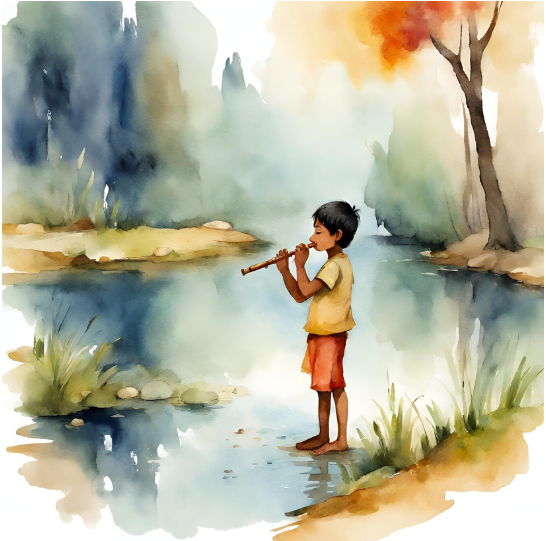
\includegraphics[scale=0.3]{tuttoori.png}
  \end{figure}
  \begin{stanza}
    ತುತ್ತೂರಿ ಊದುತ ಕೊಳದ ಬಳಿ \verseline
    ನಡೆದನು ಕಸ್ತೂರಿ ಸಂಜೆಯಲಿ \verseline
    ಜಾರಿತು ನೀರಿಗೆ ತುತ್ತೂರಿ \verseline
    ಗಂಟಲು ಕಟ್ಟಿತು ನೀರೂರಿ
  \end{stanza}
  \begin{stanza}
    ಸರಿಗಮ ಊದಲು ನೋಡಿದನು \verseline
    ಗಗಗಗ ಸದ್ದನು ಮಾಡಿದನು \verseline
    ಬಣ್ಣವು ನೀರಿನ ಪಾಲಾಯ್ತು \verseline
    ಬಣ್ಣದ ತುತ್ತೂರಿ ಬೋಳಾಯ್ತು
  \end{stanza}
  \begin{stanza}
    ತುತ್ತೂರಿ ಬಣ್ಣವು ಹಾಳಾಯ್ತು \verseline
    ಜಂಭದ ಕೋಳಿಗೆ ಗೋಳಾಯ್ತು
  \end{stanza}
\end{poem}
\end{document}
